\documentclass{article}
\usepackage[utf8]{inputenc}
\usepackage{graphicx}

\begin{document}
\title{Day 5}

\author{\emph{Teemu Sarapisto}}
\maketitle

\def\code#1{\texttt{#1}}
\newcommand{\aaa}[3]{%
  \fbox{\includegraphics[height=30mm]{#1}} \quad
  \fbox{\includegraphics[height=30mm]{#2}} \quad
  \fbox{\includegraphics[height=30mm]{#3}} \par}
\newcommand{\bbb}[3]{%
  \medskip\noindent\aaa{#1}{#1-#2}{#1-#3}}

\newpage

\setlength{\fboxsep}{0pt}%

\section{Hands-on}
\begin{figure}[h]
    \centering
    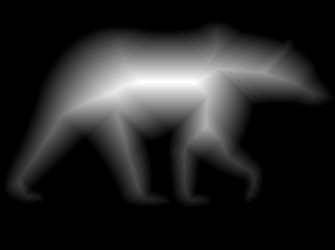
\includegraphics[scale=1.0]{distanced_bear}
\end{figure}

\subsection{Create the object skeleton with OpenCV’s ximgproc.thinning() function from the original image and try if different values for the thinningType argument would make any difference}
Main difference was that some of the thinners didn't create 1px wide lines.

\subsection{Graphing}
\fbox{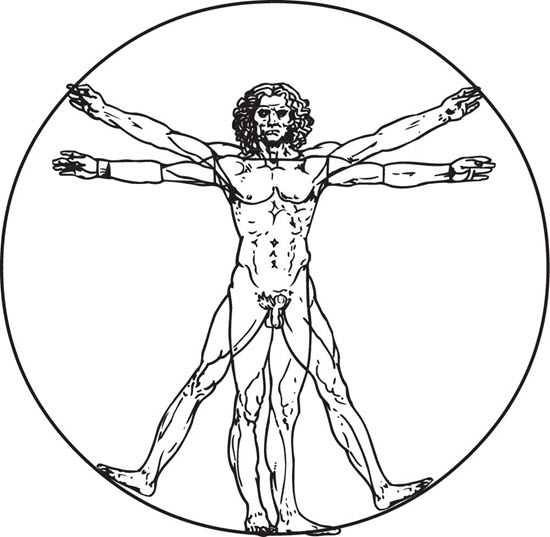
\includegraphics[scale=0.35]{da_vinci_vitruve}} \quad
\fbox{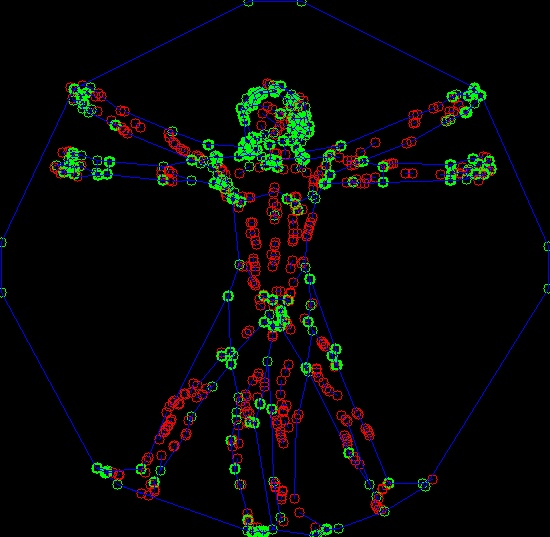
\includegraphics[scale=0.35]{vitruve}} \quad


\fbox{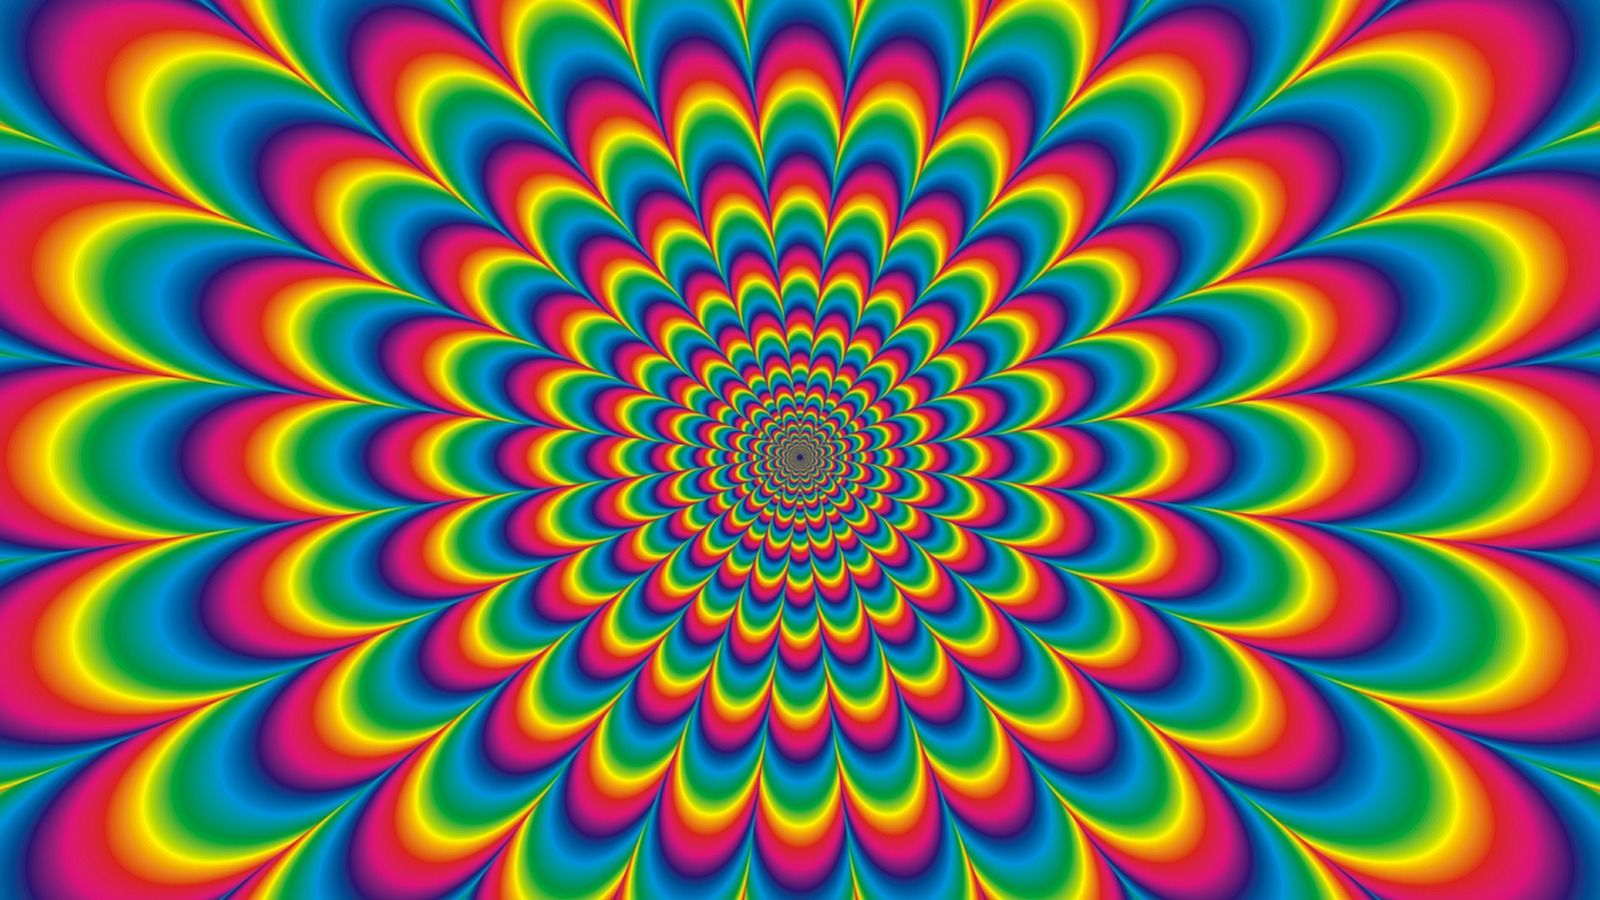
\includegraphics[scale=0.14]{psychedelic_pattern}} \quad
\fbox{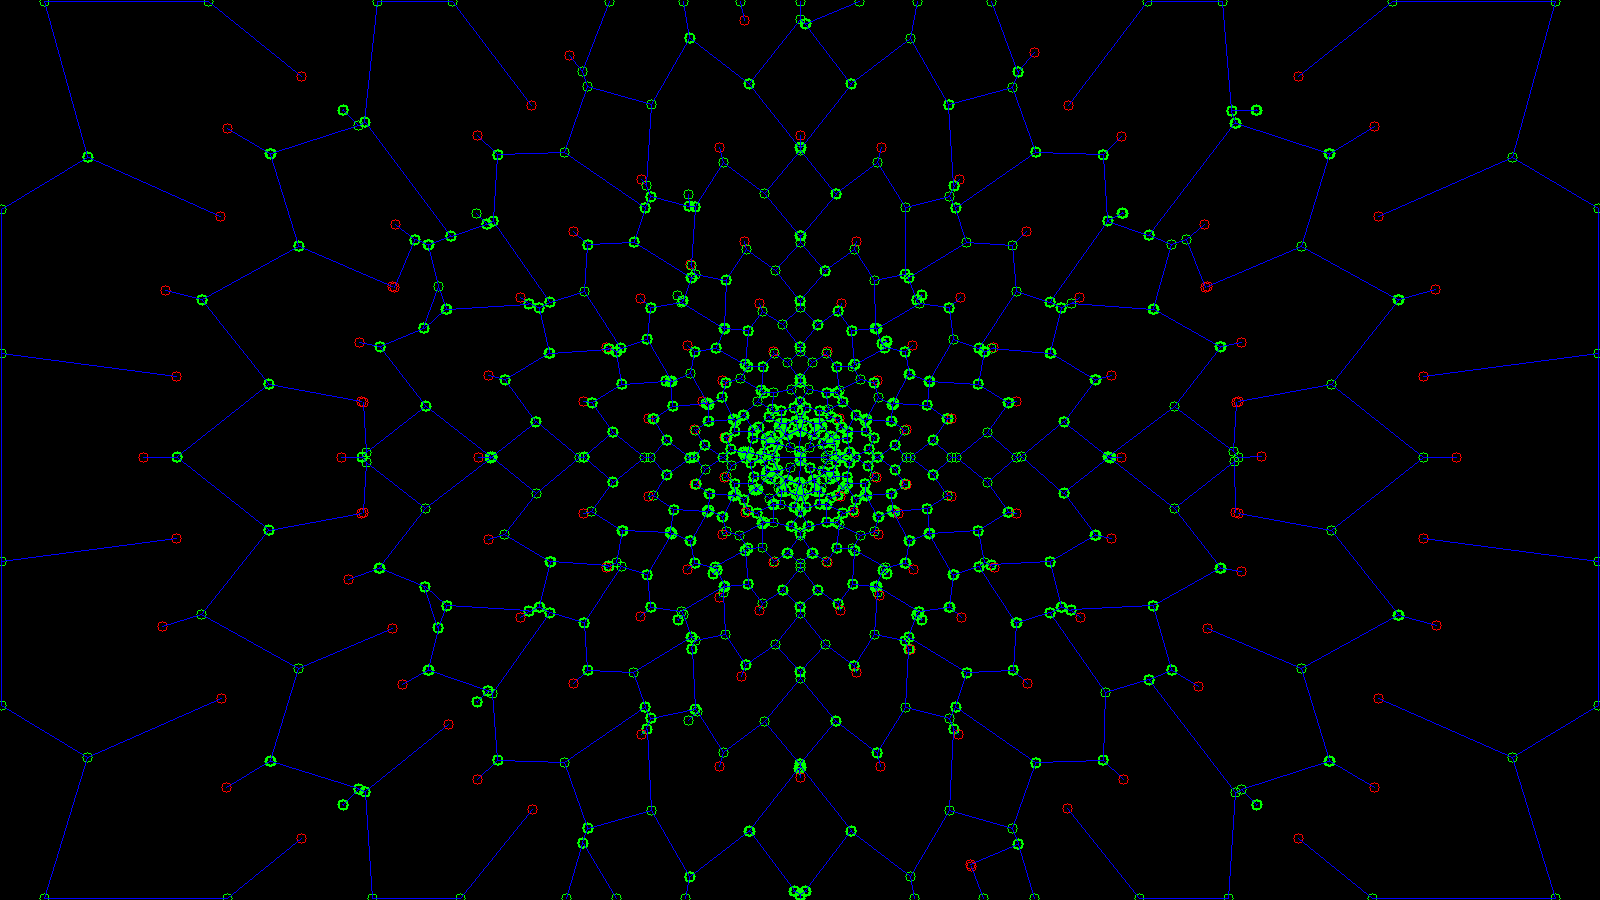
\includegraphics[scale=0.14]{psyke}} \quad

\fbox{
\includegraphics[scale=1.00]{woman_with_umbrella}} \quad
\fbox{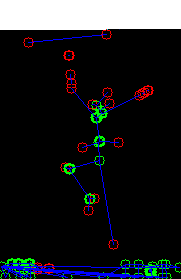
\includegraphics[scale=1.00]{umbrella}} \quad

\fbox{
\includegraphics[scale=0.25]{sacred_derp}} \quad
\fbox{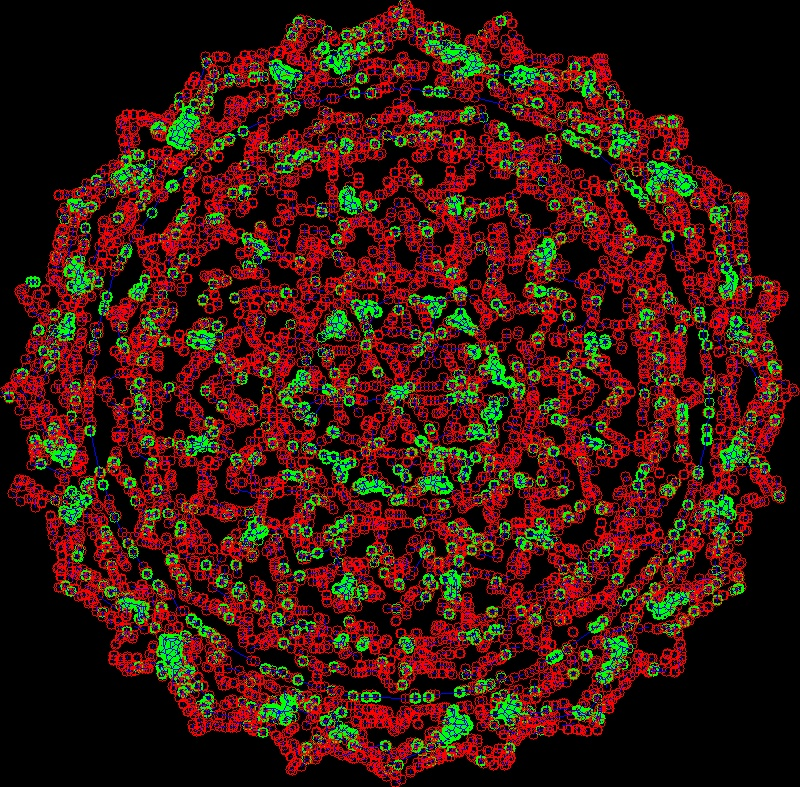
\includegraphics[scale=0.25]{sacred_graph}} \quad

\fbox{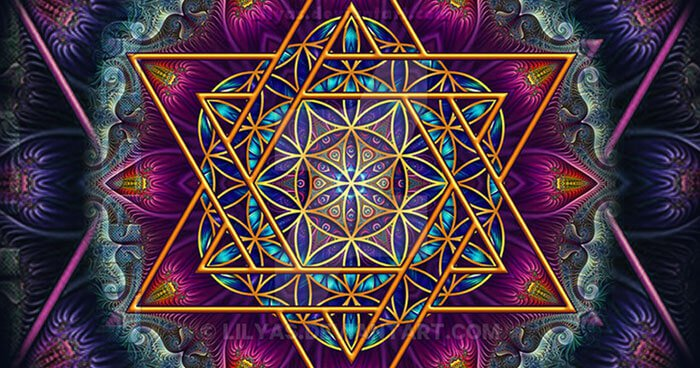
\includegraphics[scale=0.50]{sacred_2}} \quad
\fbox{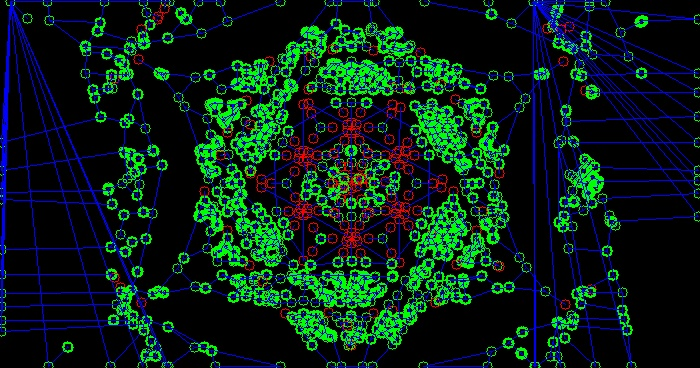
\includegraphics[scale=0.50]{sacred_graph3}} \quad

\subsection{How long it took}
around 4 hours


\end{document}
%  LocalWords:  Jorma Laaksonen pdf py tex OpenCV libopencv dev jpg
%  LocalWords:  highgui imgproc imgcodecs greyscale png opencv ing
%  LocalWords:  texlive includegraphics Exactum Gür Ersalan
